In this project it is our task to implement a circuit on the FPGA board, that can display a square patterns in the seven-segment LED display. This pattern must be able to  circulated the display both clockwise and counterclockwise.

\begin{figure}[!htbp] 
	\centering 
		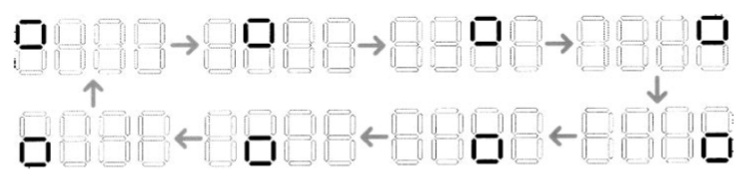
\includegraphics[scale=0.4]{fig/DigitBox.jpg} 
	\caption{Moving square on 7-segment display}
	\label{fig:1} 
\end{figure}

The circuit will switch directions dependently to the position of Switch1 and Button1 will act as reset for the system. A clock should be implemented with a slow running clock generator to display the "Moving square box". And this circuit will be implemented at both Logic Gate Level and Register Transfer Level.   
